

\documentclass[12pt]{article}
\setlength{\headheight}{14.49998pt}
\usepackage[margin=1in]{geometry} 
\usepackage[T1]{fontenc}
\usepackage{amsmath,amsthm,amssymb,amsfonts, fancyhdr, color, comment, graphicx, environ}
\usepackage{xcolor}
\usepackage{mdframed}
\usepackage[shortlabels]{enumitem}
\usepackage{indentfirst}
\usepackage{hyperref}
\usepackage{subcaption}

\renewcommand{\footrulewidth}{0.8 pt}
\hypersetup{
    colorlinks=true,
    linkcolor=blue,
    filecolor=magenta,      
    urlcolor=blue,
}


\pagestyle{fancy}


\lhead{Mila Lukić}
\rhead{Računarstvo i društvo} 
\chead{\textbf{}}
\rfoot{Matematički fakultet}

\begin{document}
\title{\Large Kurs: Računarstvo i društvo  \\[0.5cm]
        \bf\Large OSINT - Lupa u moru}
\author{\large Autor: \bf Mitar Avramović\\ \ \\}
\date{\large Datum: \today}

\makeatletter
    \begin{titlepage}
        \begin{center}
	    {\ \\ \ \\}
        \vbox{}\vspace{5cm}
            {\@title }\\[3cm] 
            {\@author}
            {\large Predmetni profesor: \bf Doc. dr Sana Stojanović Đurđević\\  \ \\}
            {\@date\\}

        \end{center}
    \end{titlepage}
\makeatother

\tableofcontents

\newpage

\section{Uvod}
\begin{text}
Od pametnih telefona u našim džepovima do algoritama koji predvi\dj aju i oblikuju naša iskustva na internetu, 
računarstvo i informatika imaju veliki uticaj na svet oko nas i budućnost tog sveta.

Uprkos ogromnom potencijalu ovog polja, postoji očigledna neuskla\dj enost po pitanju toga koji ljudi dobijaju priliku da grade ovu budućnost: žene su nedovoljno zastupljene u računarstvu.

Ovo ne samo da ometa potencijal žena u ovom polju, već i ograničava kreativnost i raznolikost mišljenja koja bi mogla pokrenuti još veći napredak i razvoj tehnologije.

Prema istraživanjima sprovedenim 2019. godine, žene predstavljaju svega 25\% radne snage u oblasti računarstva i informatike u svetu, tvrdi Liz Simons, pisac za veb sajt "computerscience.org".

Me\dj utim, ovo nije uvek bio slučaj. Prema članku sa sajta "digitalfuturesociety.com", sredinom 80tih godina prošlog veka, 50\% ljudi sa diplomom iz ove nauke u Sjedinjenim Američkim državama bile su žene. Taj broj je spao na samo 15\% u dvadesetom veku.
\end{text}

\newpage

\section{Žene i njihovi doprinosi na polju računarskih nauka}
\begin{text}
Kao što je već spomenuto, programiranje i računarske nauke tokom 20tog veka uopšte nisu imale dominantno muške radnike i naučnike. Štaviše, tokom 1940tih, programiranje se smatralo tradicionalno "ženskim" poslom! Muškarci su razvoj softvera smatrali dosadnom, napornom i inferiornom naukom, i smatralo se da je razvoj hardvera oblast sa mnogo većim potencijalom za budućnost - zato su se češće bavili time.

U današnjem dobu, mnogim mladim ljudima je teško da zamisle vreme kada razvoj softvera nije bio dominantno muški posao. Nije ni čudo što je broj žena koje ulaze u ovu industriju značajno manji. Pozitivni uzori i reprezentacija su bitan aspekat pri odlučivanju kojim poslom želimo da se bavimo, i zato je bitno obrazovati mlade o ženskim doprinosima, i inspirisati ih da i same požele da budu deo te grupe. 

U daljem tekstu biće navedene neke od žena koje su napravile značajne doprinose za istoriju računarstva.
\end{text}


\subsection{Ada Lavlejs}
\begin{text}
Ada Lavlejs (eng. Ada Lovelace, rođena kao Ada Byron) smatra se prvim programerom u istoriji. Još kao dete, Ada je pokazala sklonosti ka matematici. Učila je od jednog od najuticajnijih matematičara tog vremena, Augustusa De Morgana (eng. Augustus De Morgan), sa kojem je obra\dj ivala razne napredne teme. Jedna od njih bili su Bernulijevi brojevi.
\end{text}

\begin{figure}[htp]
    \centering
    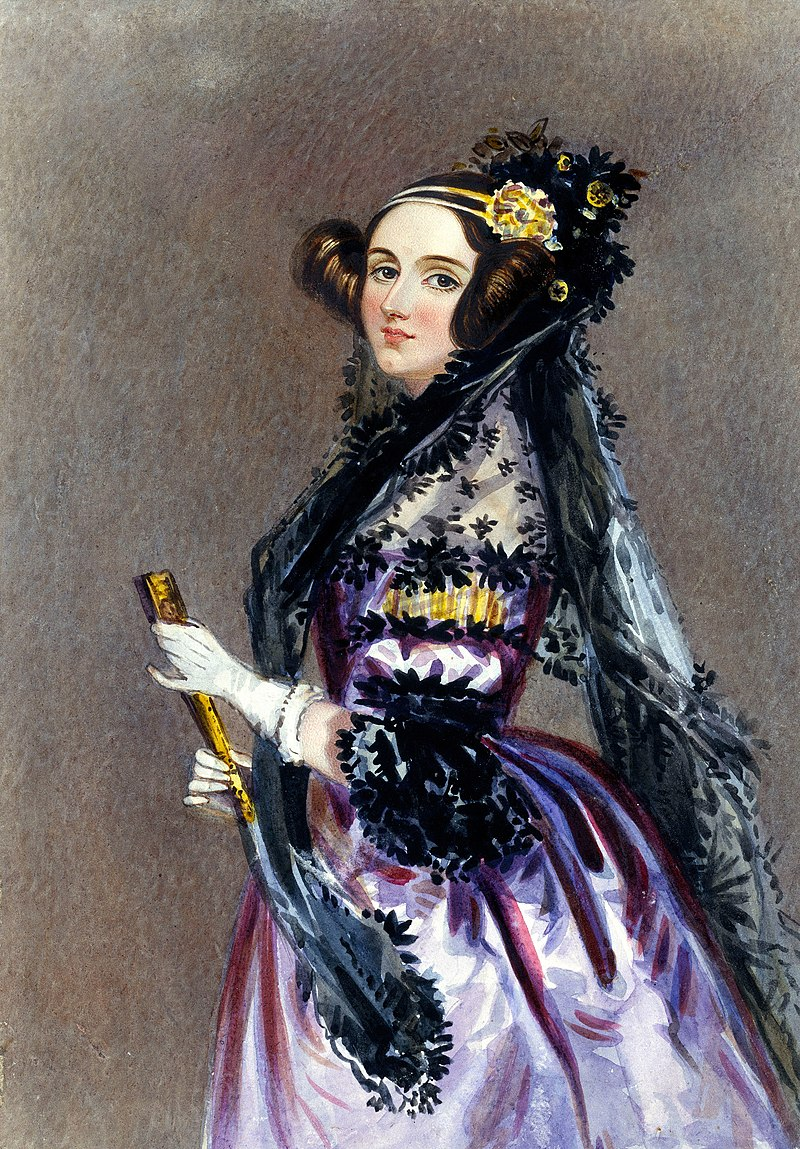
\includegraphics[width=0.4\linewidth]{image.png}
    \caption{Portret Ade Lavlejs, 1840, vodene boje}
\end{figure}

\begin{text}
Adina interesovana nisu bila ograničena samo na matematiku. Njeni prvi doprinosi u svetu računara bili su tokom rada sa Čarlsom Bebidžom (eng. Charles Babbage) na njegovoj analitičkoj masini. Pisala je pisala detaljne beleske koje su opisivale sve što je ta mašina mogla da uradi. Me\dj u njima je na\dj en i prvi računarski program: algoritam kojim se računaju Bernulijevi brojevi.

Pored toga što je autorka prvog napisanog programa, Ada je tako\dj e bila i vizionarka. Pisala je o analitičkoj mašini i njenom potencijalu da u budućnosti postane mašina koja ne samo da može da se bavi brojevima, već i ozbiljnijim problemima opšte namene.
\end{text}

\subsection{Razvoj ENIAC računara}
\begin{text}
ENIAC je bio prvi elektronski računar za opštu namenu, preteča savremenih PC-eva. Napravljen je tokom Drugog svetskog rata, kao tajni projekat američke vojske. Šest meseci nakon završetka rata, odlučeno je da se projekat podeli sa javnošću. Međutim, matematičarke koje su pisale programe na ENIAC-u su jako dugo ostale u senci. 

\begin{figure}[htp]
    \centering
    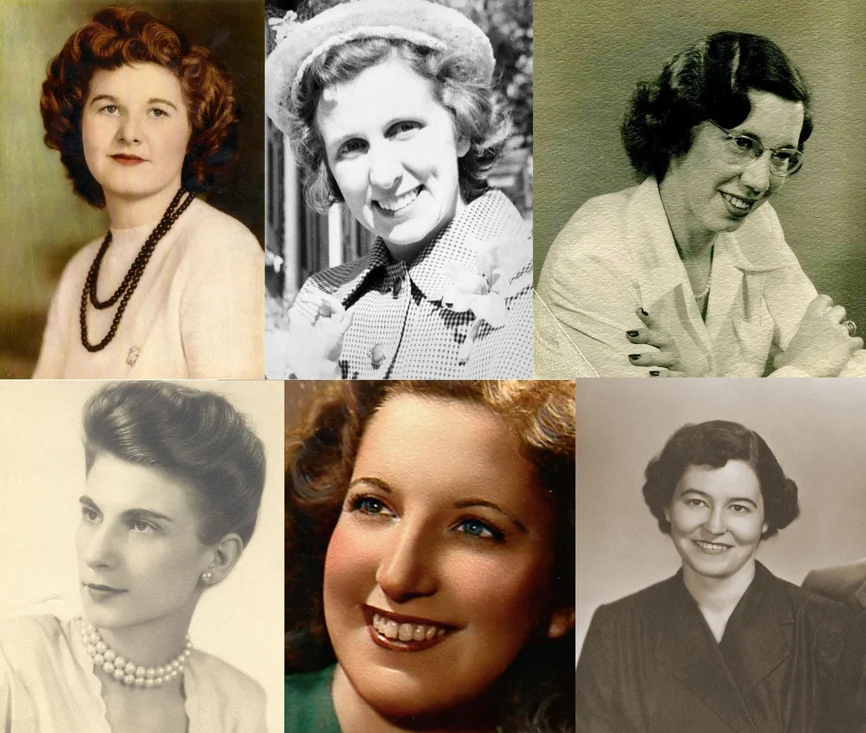
\includegraphics[width=0.9\linewidth]{eniacwomen.png}
    \caption{U smeru kazaljke na satu, počevši od gornje leve slike: Jean Bartik, Kathleen Antonelli, Betty Holberton, Ruth Teitelbaum, Marlyn Meltzer, Frances Spence}
\end{figure}

Priča o ovih šest žena: Ketlin Antoneli, Dzin Bartik, Beti Holberton, Merilin Meltzer, Fransis Spens, i Rut Tejtelbaum, podeljena je u knjizi "Proving Ground: The Untold Story of the Six Women Who Programmed the World’s First Modern Computer" koju je napisala Keti Klejnman. 
\end{text}


\subsection{Grejs Hoper}
\begin{text}
Grejs Hoper (eng. Grace Hopper) bila je američka informatičarka i matematičarka. Poput njene prethodnice Ade Lavlejs, i Grejs Hoper je zapamćena kao vizionarka. U to vreme, računarski kod se pisao na mašinskom jeziku, što je bilo jako nepraktično i naporno za programere. Grejs Hoper je predložila rešenje - pisanje koda na engleskom jeziku, i pronalaženje načina da se taj kod obradi tako da računar može da ga razume. Ovaj predlog je bio odbijen, ali je odlučila da samostalno radi na njemu.

1952. godine, Grejs Hoper je imala funkcionalni prototip kompilatora. U intervjuu za Jejl Univerzitet (Yale University), izjavila je: "Imala sam funkcionalni kompilator i niko nije želeo ni da ga pipne. Svi su mi uporno govorili da računari mogu samo da rade aritmetiku."

Pored prvog kompilatora, tako\dj e joj se pripisuje i zasluga za pronalazak prvog baga i prvo debagovanje - u pitanju je bio moljac koji se upetljao u žice računara UNIVAC-a na kojem je radila, izazivajući kratak spoj. 

\begin{figure}[htp]
    \centering
    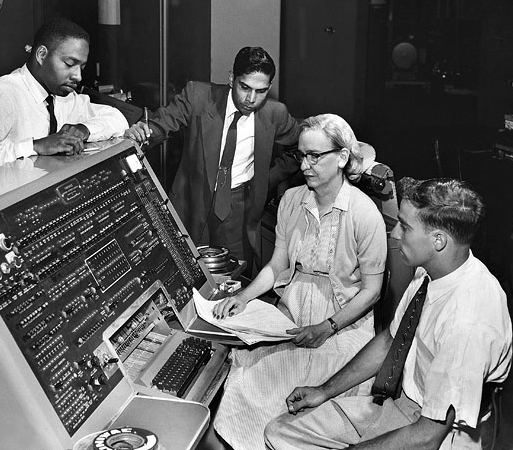
\includegraphics[width=0.8\linewidth]{gracehopper.png}
    \caption{Grejs Hoper i UNIVAC I, 1960}
\end{figure}

\end{text}

\subsection{Sestra Meri Kenet Keler}

Sestra Meri Kenet Keler (eng. Sister Mary Kenneth Keller) bila je američka edukatorka i pionir računarskih nauka. Poznata je kao jedna od prvih žena koja je doktorirala u oblasti računarskih nauka, kao i prva osoba koja je to postigla na svom univerzitetu (Univerzitet Viskonsin-Medison).

Pored toga, ostvarila je značajan doprinos pri razvoju BASIC jezika.

\begin{figure}[htp]
    \centering
    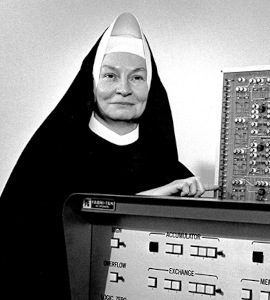
\includegraphics[width=0.6\linewidth]{marykenneth.png}
    \caption{Meri Kenet Keler}
\end{figure}

\newpage

\section{Trenutna pozicija žena u računarstvu}

Kao što je spomenuto u prethodnom poglavlju, žene su jako dugo dominirale sferom razvoja softvera i bile su pioniri u programiranju. Međutim, nekoliko događaja je doprinelo preokretu na tom polju.

\subsection{Kraj Drugog svetskog rata i testovi ličnosti za programere}

Nakon završetka Drugog svetskog rata, mnoge kompanije su shvatile da je razvoj softvera izuzetno bitna, ali i veoma skupa disciplina. Zbog toga se javlja potreba za pronalaženje "idealnog programera", odnosno osoba za koje se smatra da ima uro\dj ene predispozicije da bude dobra u ovom poslu. Dva psihologa, Vilijam Kanon i Dalas Peri (eng. William Cannon, Dallas Perry) sastavili su "Test ličnosti za programere". 

Ovaj test ličnosti je bio veoma pristrasan prema jednom specifičnom tipu ljudi: Introvertnim muškarcima koji su "opsednuti rešavanjem problema". Jedna od bitnih stavki u izveštaju bila je i da "Programeri ne bi trebalo da vole ljude". Ovom testu se pripisuje začetak stereotipa o programerima  kao asocijalnim, povučenim muškarcima. Od 1400 ljudi koji su ga "položili", 1200 su bili muškarci.

Veliki broj žena dobio je otkaze u korist muškaraca koji imaju više navodnih "urođenih predispozicija" za ovaj posao. 

\subsection{1980te: Kompjuteri kao igračke za dečake}

Vendi Hol (eng. Wendy Hall), profesorka informatike na Univerzitu u Sauthamptonu (eng. University of Southampton), zapazila je da se broj žena zainteresovanih za informatiku značajno smanjio usled pojave reklama u kojima se računari predstavljaju kao igračke za dečake i način da se sinovi i očevi zbliže.

\begin{figure}[htp]
    \centering
    \includegraphics[width=0.4\linewidth]{computerforboys.png}
    \caption{Reklama za računare iz 80tih}
    \label{fig:enter-label}
\end{figure}

\subsection{Seksizam na radnom mestu}

Istraživanje na Tehnološkom institutu u Masačusetsu 1991. pokazalo je da veliki broj žena u informatici odustaje od ove discipline ili ni ne ulazi u nju zbog mnogoprisutnog seksizma i rodnih predrasuda na radnom mestu. Ovo je i danas problem: Istraživanja pokazuju da 56\% žena napušta industriju, što je duplo češće nego muškarci. Razlozi koje navode su: 

\begin{itemize}
    \item Manjak prilika za napredovanje: Žene zauzimaju oko 30\% juniorskih, a samo 10\% seniorskih pozicija
    \item Niža zarada: Žene u IT industriji u Americi zarađuju 18\% manje od muškaraca na istim pozicijama
    \item Kultura kompanije: Čak 78\% žena tvrdi da je iskusilo seksističke, neprikladne komentare od strane kolega u firmi. Jedan od najpoznatijih primera ove pojave je esej pod nazivom "Guglova ideološka soba odjeka" (Google's ideological echo chamber), koji je napisao bivši Guglov programer 2017. godine. Ovaj esej je bio reakcija na predavanje o inkluzivnosti i diverzitetu na radnom mestu, i sadrži brojne komentare o ženskoj inferiornosti kada je u pitanju razvoj softvera. 
\end{itemize}

\subsection{Žene u računarstvu u svetu}

Iako je globalno procenat žena u računarstvu svega 25\%, a najniži u Sjedinjenim Američkim državama sa 19\%, procenti nisu ovoliko niski u svakoj državi.

U Evropi je procenat ženske radne snage u industriji dosta viši, a najveću zastupljenost imaju u Rumuniji i Bugarskoj, sa oko 60\% programerki. 

U Srbiji je procenat žena koji se bavi programiranjem u industriji oko 20\%. Bitno je naglasiti da je procenat žena koje studiraju informatiku veći. Predviđa se da će u narednih 5 do 10 godina ovaj broj porasti na 40\%.

\newpage

\section{Problemi koji nastaju zbog manjka reprezentacije u informatici}

Manjak žena u računarskim naukama nije problem samo za žene, već i za ostatak sveta. U daljem tekstu biće navedeni neki od problema sa kojima se društvo susreće zbog manjka reprezentacije u timovima koji razvijaju nove tehnologije.

\subsection{Manjak perspektiva}

Korisnici softvera nisu samo muškarci, ali se veliki broj aplikacija razvija samo sa njima na umu. Neki od poznatih primera su Voice Asistenti koji ne prepoznaju ženske glasove jer su trenirani uglavnom na muškim glasovima, kao i razni zdravstveni softveri koji bolje procenjuju stanje muškarca, tako\dj e zbog nebalansiranih skupova podataka za trening.

\subsection{Algoritamske predrasude i diskriminacija}

Algoritmi Veštačke inteligencije nisu imuni na predrasude. Skupovi za trening ovih algoritama su napravljeni na osnovu stvarnog života, te će uvek preneti i odre\dj ene stereotipe koje sa sobom nosi stvaran život. Zbog ovoga, na primer, mnogi softveri za pregledanje CV-eva i prijava za posao imaju naklonjenost ka muškim kandidatima.

\subsection{Odliv Mozgova}

Kako je već pomenuto, više od polovine žena u ovoj industriji napusti svoj posao u roku od 10 godina svoje karijere. Ovo dovodi do takozvanog "odliva mozgova" (eng. Brain Drain). Industrija gubi sposobne radnice, koje bi značajno mogle doprineti novim tehnološkim otkrićima.

\subsection{Manjak zainteresovanih korisnika}

Mnoge firme imaju problem da privuku ženske korisnike. Ovo je povezano sa manjkom perspektiva koji smo malopre spomenuli: nedostatak žena koje rade na nekoj aplikaciji vodi do toga da ta aplikacija više odgovara muškim potrebe. Lako se mogu propustiti nedostaci na tržištu.


\newpage
\section{Programi za ohrabrivanje žena u računarskim naukama}

Kako postoji očigledan manjak zainteresovanosti žena za bavljenje programiranjem, uglavnom nastao usled spoljnih uslova, osnovano je mnoštvo organizacija koje pokušavaju da smanje ovaj jaz me\dj u polovima.

\subsection{Programi namenjeni devojčicama školskog uzrasta}

Ovih programa dalje nema u Srbiji, ali postoje internacionalni programi koji se bave ohrabrivanjem devojčica u osnovnim i srednjim školama, kao i njihovo približavanje svetu programiranja. Neki od njih su "\textbf{Girls Who Code}" i "\textbf{Black Girls Code}", oba nastala u Sjedinjenim Americkim državama.

Ovi programi devojčicama i devojkama omogućuju uvodne kurseve u programiranje, letnje kampove i programe, kao i sesije sa mentorkama.

\begin{figure}[htp]
    \centering
    \begin{subfigure}{.5\textwidth}
        \centering
        
\includegraphics[width=0.5\linewidth]{gwc.png}
        \caption{Girls Who Code}
    \end{subfigure}

    \begin{subfigure}{.5\textwidth}
    \centering
    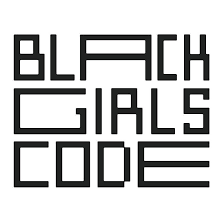
\includegraphics[width=0.5\linewidth]{gbc.png}
    \caption{Black Girls Code}
    \end{subfigure}
\end{figure}

\subsection{Programi namenjeni studentkinjama}

Ovih programa definitivno ima najviše. Omogućuju studentkinjama informatike i računarstva da se međusobno povežu, uče novije jezike i tehnologije koji obično nisu u fakultetskim programima, kao i brojne stipendije i ponude za prakse.

Neki od ovih programa su:
\begin{itemize}
    \item Ada Developers Academy
    \item AnitaB.org Institute
    \item IEEE Women in Engineering (WIE)
    \item Women in Tech (WIT)
    \item TechLadies
    \item TechWomen
    \item Women Who Code
\end{itemize}

\subsection{Programi unutar IT firmi}

Mnoge firme imaju svoje interne programe koji služe da manje zastupljenim grupama omoguće da stvore zajednicu i atmosferu u kojoj ljudi iz te manjine mogu da se međusobno osnaže i podrže. Neki od ovih programa su Google-ov "\textbf{Women @ Google}" program, koji pored pomaganja ženama unutar firme tako\dj e organizuje algoritamska takmičenja i hakatone za studentkinje, a nudi im i godišnje stipendije.

U Srbiji postoji organizacija unutar Microsofta pod nazivom "\textbf{Women know IT}", koja promoviše programiranje i svet tehnologije devojkama i organizuje konferencije i slične dogadjaje za žene.

Italijanska firma \textbf{Bending Spoons} svake godine organizuje konferencije za žene, kao i stipendije za školarine za devojke. Ova firma je poznata po tome što tako\dj e ima programe specijalno za studente i studentkinje iz Srbije.

\begin{figure}[htp]
    \centering
    \begin{subfigure}{.5\textwidth}
        \centering
        
\includegraphics[width=0.7\linewidth]{google.png}
        \caption{Women @ Google}
    \end{subfigure}

    \begin{subfigure}{.5\textwidth}
    \centering
    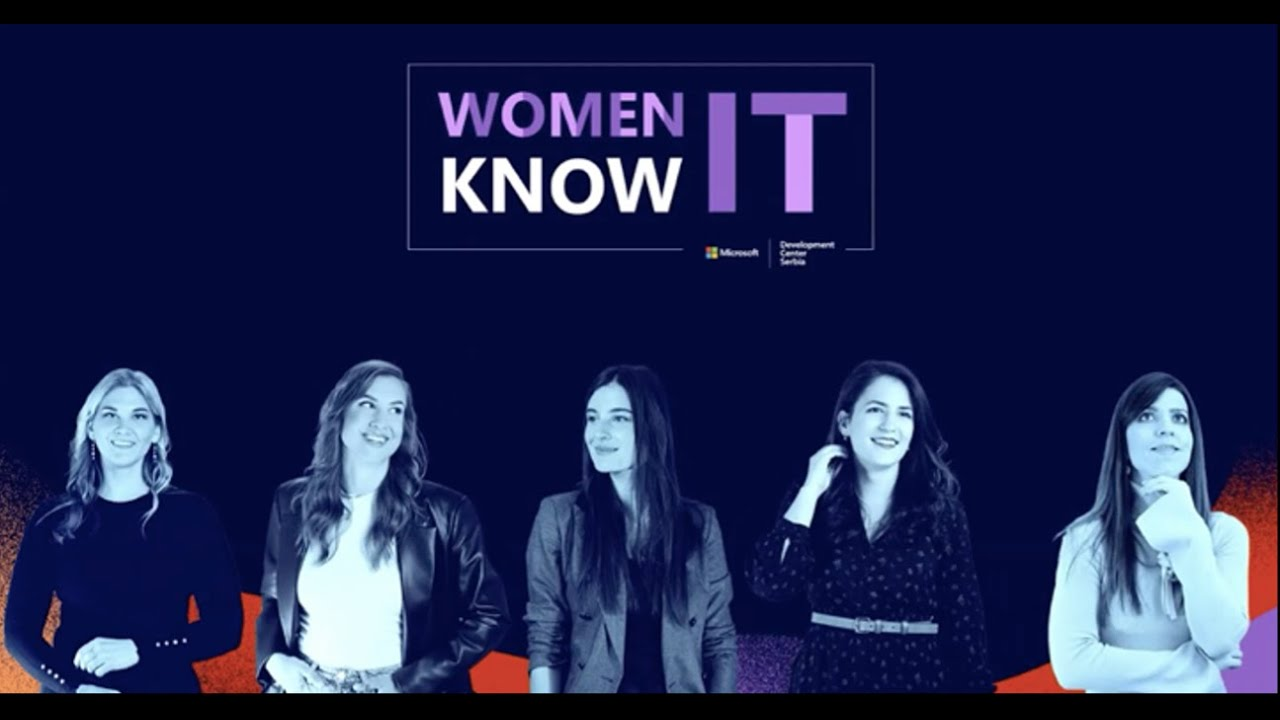
\includegraphics[width=0.7\linewidth]{womenknowit.png}
    \caption{Women know IT - MDCS}
    \end{subfigure}

    \begin{subfigure}{.5\textwidth}
    \centering
    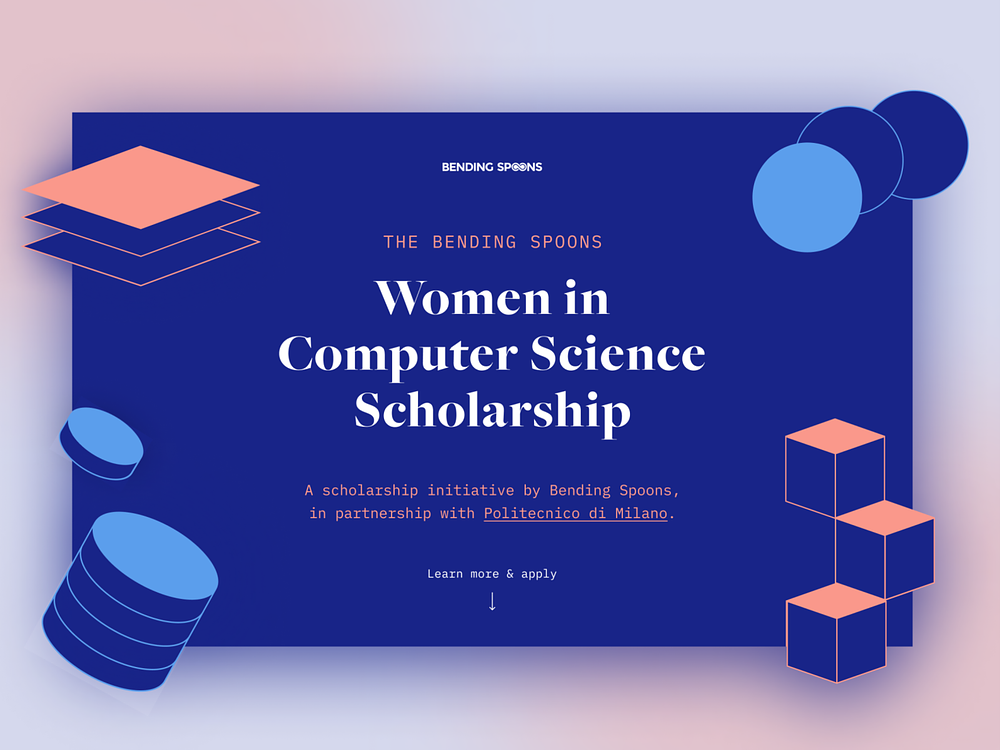
\includegraphics[width=0.7\linewidth]{bendingspoons.png}
    \caption{Bending Spoons stipendije}
    \end{subfigure}
\end{figure}

\newpage

\section{Zaključak}

Žene su bile pioniri programiranja, ostavljajući ogroman trag na istoriju računarstva. Nažalost, istorija se donekle izbrisala i mlade devojke i devojčice ne znaju za pozitivne uzore u istoriji koji bi ih inspirisali da se ovom naukom bave. Ovome ne pomaže ni činjenica da su programeri u popularnim filmovima i serijama stereotipično prikazani kao introvertni, asocijalni muškarci. Međutim, razni programi i pokreti osnovani su kako bi se ova oblast ponovo približila ženama, a vidimo i njihov značajan porast interesovanja za studiranjem informatike i računarstva u poslednjih nekoliko godina. 

Žene su potrebne u ovoj nauci, isto koliko i muškarci, jer široka reprezentacija u timovima omogućuje veću kreativnost i više inovacija za budućnost, čime se dolazi i do uvažavanja potreba svakog potencijalnog korisnika.

\newpage
\section*{Reference}
\begin{itemize}
  \item \href{https://www.computerscience.org/resources/most-influential-women-computer-science}{Most Influential Women in Computer Science - computerscience.org}  
  \item \href{https://digitalfuturesociety.com/programming-when-did-womens-work-become-a-mans-world/}{Programming: When did women's work become a man's world? - digitalfuturesociety.com} 
  \item  \href{https://poincare.matf.bg.ac.rs/~ivana/tnp2022/reviews/18_VelickovicZagoracBigovicJevtic_review.pdf}{Žene u programiranju - Seminarski rad na Matematičkom fakultetu, Jelena Veličković, Bojana Zagorac, Miloš Bigović, Zorana Jevtić (TNP, 2022)}
  \item  \href{https://en.wikipedia.org/wiki/Ada_Lovelace#First_published_computer_program}{Ada Lovelace - Wikipedia}
  \item  \href{https://spectrum.ieee.org/the-women-behind-eniac}{The Women Behind ENIAC - Joana Rich}
  \item  \href{https://en.wikipedia.org/wiki/Grace_Hopper#World_War_II}{Grace Hopper - Wikipedia}
  \item  \href{https://www.cs.yale.edu/homes/tap/Files/hopper-wit.html}{"The Wit and Wisdom of Grace Hopper" - Yale University}
  \item  \href{https://en.wikipedia.org/wiki/Mary_Kenneth_Keller}{Mary Kenneth Keller - Wikipedia}
  \item  \href{https://en.wikipedia.org/wiki/Women_in_computing}{Women in Computing - Wikipedia}
  \item  \href{https://dl.acm.org/doi/pdf/10.1145/1142620.1142628}{A VOCATIONAL INTEREST SCALE FOR
COMPUTER PROGRAMMERS - William Cannon and Dallas Perry}
  \item  \href{https://www.womenintech.co.uk/6-reasons-why-so-many-women-leave-tech-jobs/#:~:text=A%20staggering%2056%25%20of%20women,this%20percentage%20will%20only%20decrease.}{Why Women leave Tech}
  \item  \href{http://ns2.matf.bg.ac.rs/~milena/msnr/2022/finalne_verzije/03_ProblemiRodneRavnopravnostiUInformaticiUSvetu_AleksicMarkovicKeljacJovicic.pdf}{Problemi rodne ravnopravnosti u informatici u svetu - Seminarski rad u okviru kursa Metodologija strucnog i naucnog rada, Andrijana Aleksić, Bogdan Marković, Jelena Keljać, Luka Jovičić}
  
  \item
  \href{https://en.wikipedia.org/wiki/Google%27s_Ideological_Echo_Chamber#Cultural_commentary}{Google's Ideological Echo Chamber - Wikipedia}
  \item
  \href{https://www.cio.com/article/215709/16-organizations-for-women-in-tech.html}{20 Organizations for Women in Tech - cio.com}
\end{itemize}

\end{document}